While the last chapter has shown the application of a neural network for a simple use case, 
this chapter will go into more detail on the different parts of such a model and its configuration.

The fact that this model incorporates numerous processing units that compute a single output which is passed on to other units was inspired by the brain's computational mechanism, 
though to compare it to the real neural system in human brains makes an overly simplistic assumption on our cognitive system and is not accurate and just the naming convention has stuck \citep{goldberg2017neural}.

In general a neural network takes input values in form of numeric vectors.
In this thesis a single input vector will be notated by $x$. 
The training of such a model takes not one input vector at a time, but rather a so called batch which is the collection of a certain number of input vectors into a matrix where the rows represent the different samples. 
To reference the j-th value of the i-th sample in the input matrix the notation is $\textbf{X}_{i,j}$.

Next it has any number of layers which consist of an arbitrary number of processing units. 
All layers that are not the input vector or the last layer in line are called hidden layers since during computations the user does not interact with them. 
These will be referred to as $h^{(k)}$ where it is the k-th hidden layer.

Finally the layer which produces the output of the whole model is called output layer which is notated by $y$. 

If all the units between two layers are connected to each other, the network is called fully connected or affine \citep{goldberg2017neural}.

All the units take as input the outputs of connected units of the layer before, multiply them with weights $\textbf{W}$ which are specific for this layer and in most cases sum up the results of the multiplication. 
Seldom, instead of summing up the results of the multiplications, a unit could just use the maximum or some other statistics on them \citep{goldberg2017neural}.

Once this step is done the unit adds a bias $b$ and applies a non-linear function which will produce the output that will be passed on to the next layer. 
Without separating these linear combinations by these so called activation functions the whole neural network would be a long, but linear function of the input values itself. 

Activation functions transform the value as the last step of all processes done by a unit and in many cases scale its output. 

Suppose we have a batch of 100 samples with a length of their input of 20, one hidden layer with 30 units and the output layer with 10 units. Then we have the following matrices and vectors with their dimensionality:
 
\[    \textbf{X} \in {\rm I\!R}^{100 \times 20}  \]
\[    \textbf{X}_{1 .} = x^{(1)} \in {\rm I\!R}^{20}  \]
\[    \textbf{W}^{(1)} \in {\rm I\!R}^{20 \times 30}  \] 
\[    b^{(1)} \in {\rm I\!R}^{30}  \]
\[    h^{(1)} \in {\rm I\!R}^{30}  \]
\[    \textbf{W}^{(2)} \in {\rm I\!R}^{30 \times 10}  \]
\[    b^{(2)} \in {\rm I\!R}^{10}  \]
\[    y \in {\rm I\!R}^{10}  \]

If we consider a single input sample, vector $x$, we can associate the units of layers with the scalar values they return for their singular (not a batch/matrix) input and the dimensionality seen above stays correct. 
For simplicity activation functions are represented by the lower case letter 'a' and are not yet specified in more detail, but could be any function presented in \ref{nn_act}. 

\[   h^{(1)} = a_1(x\textbf{W}^{(1)} + b^{(1)})   \]
\[   y = a_2(h^{(1)} \textbf{W} + b^{(2)})   \]

If the whole batch of samples is propagated through this example neural network, the whole equation would be:

\begin{equation} 
\label{eq:1}
    a_2(a_1(\textbf{X}\textbf{W}^{(1)} + \textbf{b}^{(1)}) \textbf{W}^{(2)} + \textbf{b}^{(2)})
\end{equation}

This would result into an output with the dimensionality of $100 \times 10$ where each row represents the output of layer $y$ for one row of the input matrix \textbf{X}. In the equation with matrices the bias vectors $b^{(k)}$ are added similarly for each row of the matrix to the left side of the addition sign or can just be considered as a matrix with the same bias vector for all its rows.

Considering \textbf{X} as the beginning of the information flow through the neural network, it is first passed on through the hidden layer $h^{(1)}$ and finally through the output layer $y$. The direction of the information flow is merely forward through the different layers which motivated the naming convention for such simple models as Feed-Forward Neural Network. The flow of information can be passed back to previous layers for Recurrent Neural Network which will be defined in \ref{nn_rnn}.

In the following section four of the most important activation functions are presented.


%-------------------------------------------------------------------------------------------


\subsubsection{Activation functions}
\label{nn_act}

First of is the sigmoid $\sigma$ function, shown in equation \ref{eq:simoid}, which maps any value it receives onto the range [0,1], a property that makes this activation function attractive for the usage at an output layer where a probability for binary classification is considered useful. Additionally the effect of outliers for possible following layers is mitigated.

\begin{equation}
\label{eq:simoid}
    \sigma(x) = 1 / (1 + e^{-x})
\end{equation}


Next of is the hyperbolic tangent $tanh$ function which behaves very similarly to the sigmoid function except that it squashes the values to the range of [-1,1] and thereby maps outliers towards the mean \citep{jurafsky2021}. Its equation is the following:

\begin{equation}
\label{eq:tanh}
    tanh(x) = (e^x - e^{-x}) / (e^x + e^{-x}) 
\end{equation}

It's derivative is vanishing less quickly than the sigmoid's which is a favorable property for the training process explained in \ref{nn_train}.


Build as an approximation of the $tanh$ activation function the hard tanh $hardtanh$, shown in equation \ref{eq:htanh}, is a more computationally efficient alternative \citep{goldberg2017neural}.
    
\begin{equation}
\label{eq:htanh}
    hardtanh(x) = \begin{cases}
  -1   \text{\phantom{xx} x $<$ -1} \\
   1   \text{\phantom{xxxi} x $>$ 1} \\
   0   \text{\phantom{xxxi} otherwise.}
\end{cases}
\end{equation}
    


Finally, the Rectified Linear Unit $ReLU$ activation function which we have already seen in chapter \ref{nn_xor} is presented. 
Positive values given to this function will be returned without any modification and negative values are capped so that the smallest value this function returns is 0. This can be mathematically expressed as in equation \ref{eq:relu}. 
$ReLU$ is computationally very efficient and has nearly linear properties \citep{jurafsky2021}. 

\begin{equation}
\label{eq:relu}
    ReLU(x) = max(0, x)
\end{equation}

It's derivative is either 0 for all values less than zero or 1 for all values greater than zero. 
The property that the gradient for positive values is constantly at 1 is one advantage of $ReLU$ over the other activation functions presented here since the other functions struggle with the fact that their gradients may become infinitesimal small or are 0 for extreme values.

In figure \ref{fig:AF} the four activation functions are plotted and their respective derivatives.

\begin{figure}
  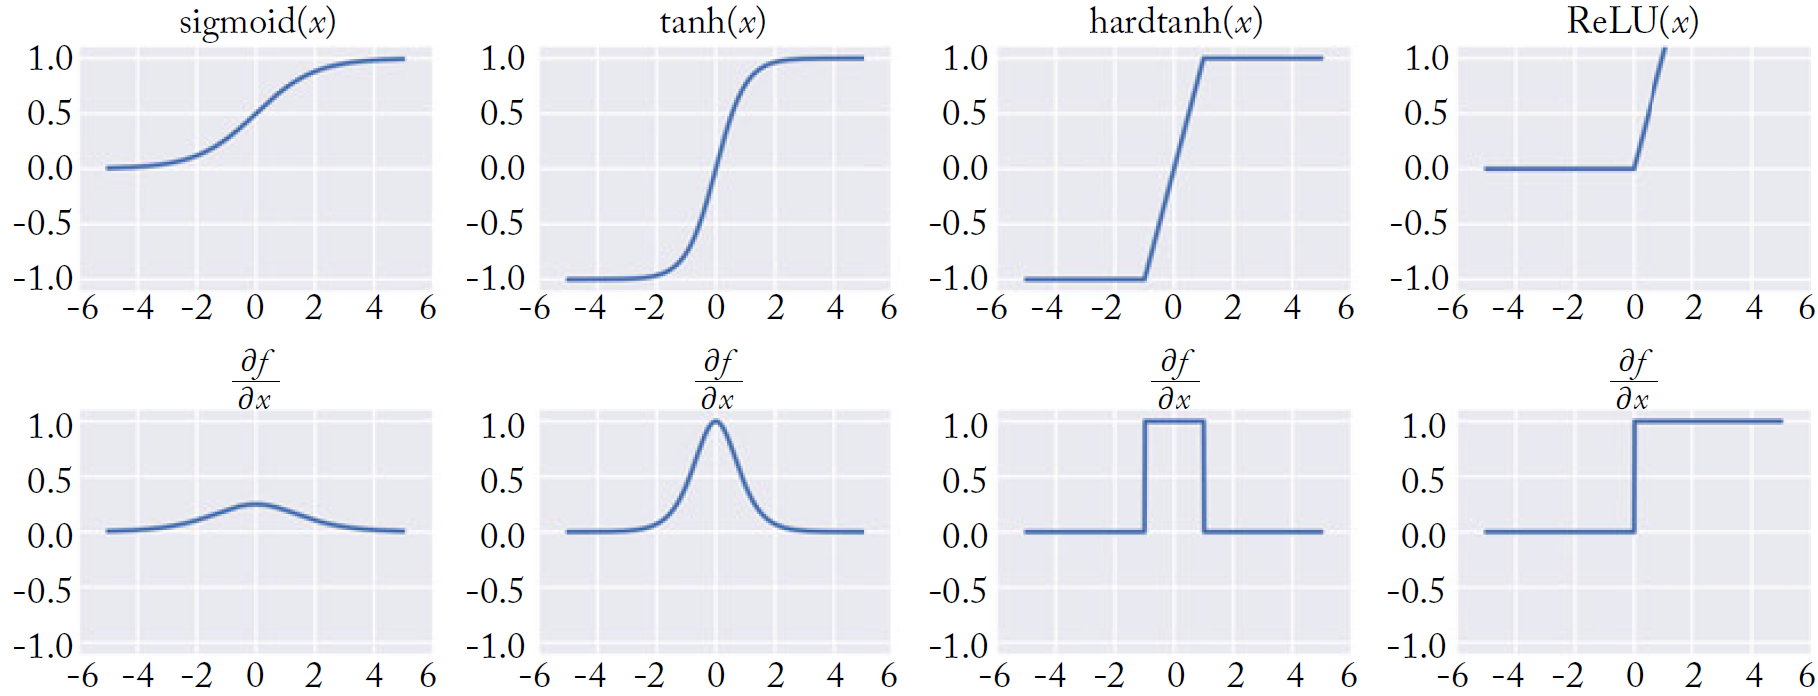
\includegraphics[width=\linewidth]{Pictures/Goldberg_17_AF.png}
  \caption{Adapted from \citet{goldberg2017neural}: Plots of the functions and their derivatives for the sigmoid, tanh, hardtanh and ReLU activation function}
  \label{fig:AF}
\end{figure}

While not strictly speaking an activation function, it's application on whole vectors of output layers make the $softmax$, shown in equation \ref{eq:softmax}, somewhat related to the functions mentioned above. 

\begin{equation}
\label{eq:softmax}
    softmax(x_i) = e^x_i / \sum_{j=1}^{C} e^{x_j}
\end{equation}

For the output layer in settings where a probability distribution over different class choices is favorable, e.g. POS-tagging, the $softmax$ function is used on the units of the output layer. 
It normalize all the values in such a way that their sum is 1 and they can be regarded as conditional probabilities for being a certain class \citep{jurafsky2021}.

In Equation \ref{eq:softmax} we suppose that the final layer has C units.


%-------------------------------------------------------------------------------------------


\subsubsection{Loss function}
As neural networks are an instance of supervised machine learning, we possess the correct output for the samples on which we train our model. 

To extract information on the model's quality on performing a certain task, we need to quantify the degree to which the model makes the right decisions. 
Therefore a so called loss function is instantiated which compares the model's output with the validated output we have on our training data and applies different metrics to make the correctness tangible.
Since the neural network usually provides a distribution as its output for a given prediction, conditioned on the input it has received and the model's parameters, the final decision is based on the principle of maximum likelihood \citep{jurafsky2021}.

This limits the scope of this thesis and its the application of the described neural networks to tasks where there is one correct output among at least two choices.
This makes the Cross-Entropy ($L_{CE}$) loss function, as seen in equation \ref{eq:cross}, a valid choice to quantify the distance between the model's decisions and the gold standard \citep{Goodfellow-et-al-2016}.

\begin{equation}
\label{eq:cross}
    L_{CE}(\hat{y},y) = \sum_{i=1}^{C} y_i log\hat{y}_i
\end{equation}

In this equation we suppose that our output is a vector of length $C$ which represents the number of possible categories from which the model has to choose. 
The gold standard that was not generated by the model is a one-hot-encoded vector in which the true class is encoded as 1, while the other positions in the vector are 0.

In cases in which we use the neural network for a binary classification task the Cross-Entropy loss function can be reduced to a function which is analogous to the loss function for a logistic regression \citep{jurafsky2021}.

One alternative loss function, though mostly used in linear regression tasks, would be the Mean Squared Error loss (MSE). It sums up the squared distances between the model's prediction and the real output for each possible class. Afterwards it is multiplied by the inverse of the number of classes ($C$) as shown in equation \ref{eq:mse}:

\begin{equation}
\label{eq:mse}
    L_{MSE}(\hat{y},y) = (1/C) * \sum_{i=1}^{C} (y_i - \hat{y}_i)^2
\end{equation}

The MSE is seldom a reasonable choice for classification tasks in neural networks. The fact that the usage of this loss function assumes the data to be derived from a normal distribution and the assumption that the values provided to the function are arbitrary real valued numbers, not restricted to the range of probabilities [0,1], makes the MSE inappropriate for most settings for which neural networks are used \citep{khan2019mse}.


%-------------------------------------------------------------------------------------------


\subsubsection{Training Neural Networks}
\label{nn_train}
So once a loss function is chosen, input data, typically in batches, can be fed into the neural network and it will pass through the consecutive layers and produce an output. 
Afterwards the loss is calculated for the model and it is possible to quantify the distance between the correct output and the predicted one. 
This flow of data through all the computations is called the forward pass \citep{goldberg2017neural}.

We can use the information the loss function provides to adjust the weights and biases, the parameters, of the model and ideally make it perform better. 
This is done by minimizing the loss and computing the partial derivatives of the loss function with respect to each parameter of the neural network and adjusting the parameters according to them \citep{Goodfellow-et-al-2016}.

Even if the loss function itself is not necessarily convex which means that there might be local minima in which the optimization might get stuck, gradient based methods like gradient descent for training a neural network are widely used and have proven to work well in practice \citep{goldberg2017neural}.

Since the model consists of several layers with a multitude of parameters each, the task of calculating the gradient can get very complex and cumbersome. 
Therefore the chain-rule of differentiation is applied to make the calculations more docile.

Often computation graphs, which are directed acyclic graphs of the partial calculations involved in computing the loss, are used to simplify the process of determining the gradient and derivatives for the model \citep{goldberg2017neural}.
Being broken down into separate operations the forward pass through the neural network will produce some additional intermediate results, but its major gain lies in the backward pass of information.

By using the chain-rule a gradient for each operation in the computation graph can be computed step by step through the directed acyclic graph by using the gradient gotten from the previous step.

The name backward pass springs from the fact that the first derivative we compute starts at the loss function itself and we move backwards through all the operations involved. This procedure is called the error backpropagation algorithm \citep{jurafsky2021}.

Since the forward pass has produced the intermediate results for all operations in the chain of equations, the derivatives are easily calculated once the partial gradients are worked out \citep{jurafsky2021}.

Afterwards these are used to adjust weights and biases of the model after being multiplied with a learning rate which tries to stabilize the training process.


